% !TEX root = ../thesis.tex

\chapter{Higher order relativistic effects in the bispectrum}
\label{chapter:ho}

In this chapter, we summarise previous work on relativistic projection effects in the observed galaxy bispectrum~\cite{Umeh:2016nuh,Jolicoeur:2017nyt,Jolicoeur:2017eyi,Jolicoeur:2018blf} going beyond the $\ord(\cH/k)$ approximation used in the previous chapters. For the bispectrum, similar to the power spectrum, effects from observing on the past lightcone need to be taken into account, as they distord the information which is contained in the underlying distribution of dark matter. These lightcone projection effects themselves can also provide new information. The major difference between the power spectrum and bispectrum analyses however, is that for the bispectrum, projection effects up to second order in perturbation theory are required. 

Previously, the GR effects on the angular bispectrum of galaxies arising from lensing convergence has been computed in~\cite{DiDio:2015bua}, which neglects other ultra-large scale GR corrections to the galaxy overdensity. In~\cite{Kehagias:2015tda}, a separate-universe approximation is used to compute the angular bispectrum of galaxies in the squeezed limit only, but including all GR lightcone effects. In Section~\ref{sec:localproj} we discuss the Fourier-space observed galaxy biscpectrum including corrections from local projection effects and relativistic corrections from nonlinear dynamical evolution on large scales, which contribute significantly. At second order in general relativity, scalar perturbations also generate second-order tensor and vector modes~\cite{Mollerach:1997up,Matarrese:1997ay}, and these modes enter the observed galaxy number density contrast at second order~\cite{Bertacca:2014hwa,Bertacca:2014wga,Bertacca:2014dra,Yoo:2014sfa,DiDio:2014lka}. However, the power in these second-order tensor and vector modes is much smaller than the power from the scalar modes, and is neglected in forthcoming chapters-- a brief discussion on the vector and tensor modes can be found in Section~\ref{sec:tensorvector}. 


\section{Local lightcone projection effects}\label{sec:localproj}

The observed galaxy bispectrum at tree level involves projection effects at both first and second order. These effects, which arise from observing on our past lightcone, include local contributions from Doppler and gravitational potential terms, integrated contributions such as lensing, and at nonlinear order there are also couplings between almost all of these projection effects. On ultra-large scales, the relativistic contributions mimic the effects of scale-dependent bias and hence they are crucial for a complete theoretical description. 

Since we work in Fourier space, which is common with much of the literature on the galaxy bispectrum, we necessarily neglect terms involving lensing and other line-of-sight integrals, i.e. only local relativistic projection effects are included. Furthermore, another approximation which is a direct consequence of working in Fourier space is the plane-parallel approximation, neglecting wide-angle correlations. These and need to be included for improved theoretical accuracy. When using an angular harmonic or three-point correlation function analysis, the wide-angle effects would be automatically included, but it poses further computational challenges~\cite{Bertacca:2017dzm}. 

To be able to compute the observed tree-level bispectrum including local projection effects, we need the observed galaxy number count contrast $\Delta_g^\tw$. The full expression for $\Delta_g^\tw$~\cite{Bertacca:2014dra,Bertacca:2014wga,Bertacca:2014hwa,Yoo:2014sfa,DiDio:2014lka} is very long and complicated, even when integrated contributions are omitted. Conveniently, when neglecting integrated contributions, a fully general form of $\Delta_g^\on$ and $\Delta_g^\tw$ can be expressed in Poisson gauge. All terms at the observer are neglected too, since they do not contribute to the bispectrum. 

Important to note is how the bispectrum is still dependent on the magnification bias, despite omitting integrated effects. This is because GR weak lensing convergence consists of both the standard integrated term and local non-integrated terms~\cite{Bonvin:2008ni}, and hence magnification bias still enters the bispectrum even when integrated terms are ignored. Previous sections have already illustrated the dependence of bispectrum power and detectability on the evolution and magnification biases, highlighting the importance of modelling these self-consistently from the same luminosity function.

The observed number density contrast $\Delta_g$ is defined through, 
\begin{equation}
	\frac{\diff N(z, \n > \ln L)}{\diff z \diff \Omega_o} = \frac{\chi^2(z)}{(1 + z)^4 \cH(z)} \bar{\N}(z, > \ln L) \left[ 1 + \Delta_g(z, \n, >\ln L) \right],
\end{equation}
where $\diff N$ is the observed count of galaxies above threshold luminosity $L$, in direction of observation $\n$, within redshift interval $\diff z$ and within solid angle element $\diff \Omega_o$. $\cH(\eta) = a'(\eta)/a(\eta)$ is the conformal hubble rate, $\bar{\N}$ is the background magnitude-limited number density, and $\chi$ is the comoving line-of-sight distance. Expanding $\Delta_g$ up to second order in perturbation theory as, 
\begin{equation}
	\Delta_g(z,\n) = \Delta_g^\on(z, \n) + \frac{1}{2} \left[ \Delta_g^\tw(z,\n) - \langle \Delta_g^\tw(z,\n)\rangle \right]\,,
\end{equation}
where we have dropped the dependence of the density contrast on luminosity for brevity, and subtract $\langle \Delta_g^\tw \rangle$ to ensure that $\langle \Delta_g \rangle = 0$. 

The observed number density contrast can be split into Newtonian and relativistic parts at each order in perturbation theory,
\begin{equation}
	\Delta_g^{(r)} = \Delta_{g \nw}^{(r)} + \Delta_{g \gr}^{(r)}\,,
\end{equation}
which is convenient for our purpose here. Since we consider the bispectrum at a fixed redshift $z$, we drop redshift dependence for convenience. 

Radial and transverse derivatives are, 
\begin{align}
	&\partial_{\parallel} = n^i \partial_i\,,\label{eq:partialparalleldef} \\
	&\partial_{\perp i} = \partial_i - n_i \partial_\parallel\,,\label{eq:partialperpdef}
\end{align}
the derivative down the past lightcone is defined as, 
\begin{equation}
	\frac{\diff}{\diff \chi} = - \frac{\diff}{\diff \eta} = - \partial_\eta + \partial_\parallel\,\label{eq:ddchidef}
\end{equation}
and the screen-space projected Laplacian is, 
\begin{equation}
	\nabla^2_\perp = \nabla^2 - \partial_\parallel^2 - \frac{2}{\chi} \partial_\parallel\,.
\end{equation}

We are free to choose the most convenient gauge for our purpose to compute $\Delta_g$, as it is an observable quantity and hence gauge-independent. Since splitting the observed number density contrast into Newtonian and relativistic parts is convenient in Poisson gauge, it is our gauge of choice. The metric and the peculiar velocity of galaxies (which on the scales of interest is equal to the peculiar velocity of the underlying dark matter distribution) are, 
\begin{align}
	a^{-2} \diff s^2 &= - \left[ 1 + 2 \Phi^\on + \Phi^\tw \right] \diff \eta^2 + \left[ 1 - 2 \Phi^\on - \Psi^\tw \right] \diff\x^2\,,\\
	v^i &= \partial^i \left[ v^\on + \frac{1}{2} v^\tw \right]\,.
\end{align}
The observed comoving coordinates of a galaxy are $\x = \chi(z) \n = [\eta_0 - \eta(z)] \n$~\cite{Bertacca:2014dra}, and we assume that anisotropic stress vanishes at first order in which case $\Psi^\on = \Phi^\on$.

The comoving-synchronous gauge (C) overdensities of matter and galaxy counts are denoted as $\delta_{m\cs}$ and $\delta_{g\cs}$. At first order, the Poisson and continuity equaitons are,
\begin{align}
	&\nabla^2 \Phi^\on = \frac{3}{2} \Omega_m \cH^2 \delta_{m\cs}^\on \\
	&\delta_{m\cs}^{\on'} = - \nabla^2 v^\on\,.
\end{align}
These lead to the following relations for the velocity and metric potentials,
\begin{equation}
	\Phi^\on = \frac{3}{2} \Omega_m \frac{\cH^2}{k^2} \delta_{m\cs}^\on\,,
\end{equation}
where $\Phi^\on(a,\k) = \frac{D(a)}{a} \Phi^\on(1,\k)$, and,
\begin{equation}\label{eq:scdepvel}
	\cH v^\on = f \frac{\cH^2}{k^2} \delta^\on_{m\cs}\,,
\end{equation}
where $f = \frac{\diff \ln D}{\diff \ln a}$ and $\delta^\on_{m\cs}(a,\k) = D(a) \delta^\on_{m\cs}(1,\k)$. 


\subsection{Observed galaxy number counts}
Working in Poisson gauge, we can split the first-order observed galaxy number counts $\Delta_g^\on$ into Newtonian and relativistic parts as, 
\begin{align}
	&\Delta_{g\nw}^\on = b_1 \delta_{m\mathrm{T}} - \frac{1}{\cH} \partial_\parallel^2 v^\on\,\label{eq:DeltagNFO}\\
	&\Delta_{g\gr}^\on = \left[ b_e - 2 \Q + \frac{2 (\Q - 1)}{\chi \cH} - \frac{\cH'}{\cH^2} \right] \left[ \partial_\parallel v^\on - \Phi^\on \right] _ (2 \Q - 1) \Phi^\on + \frac{1}{\cH} \Phi^{\on \prime} \nonumber \\
	& + (3 - b_e) \cH v^\on\,\label{eq:DeltagGRFO}.
\end{align}
In the above equation, the Newtonian part concists of the T-gauge density contrast and the Kaiser RSD. The terms in the GR part are the Doppler term which is proportional to the line-of-sight velocity $\partial_\parallel v^\on$, and terms arising from the potential and the velocity potential. 

At second order, the expression for $\Delta_g$ is a lot more involved, because it includes both the second-order generalisations of effects included at first order, as well as quadratic couplings between the first-order terms themselves. Various groups have computed the second order observed galaxy number counts, in different formalisms. A full comparison of the different results has yet to be done, see for example~\cite{Fuentes:2020qby} in which the leading order corrections are compared.

Here we use the expression given by~\cite{Bertacca:2014hwa}, which includes the evolution and magnification biases-- we neglect the integrated effects that are given, and we include our gauge-independent model of second-order galaxy bias. The resulting expression for $\Delta_g^\tw$ is, 
\begin{align} 
\Delta_{g}^{(2)} &= b_1 \delta_{m{\mathrm{T}}}^\tw + b_2 \left[\delta_{m{\mathrm{T}}}^\on \right]^2 + \left[(b_e-3)^2 \cH^2 + b_e' \cH +(b_e-3) \cH' \right] \left[v^\on \right]^2 \nonumber \\
& + (b_e - 3)\cH v^\on v^{\on \prime} + 2b_1 (3 - b_e) \cH v^\on \delta_{m\mathrm{T}}^{(1)} - 2v^\on \left[ b_1 \delta_{m\mathrm{T}}^{\on \prime} + b_1' \delta_{m\mathrm{T}}^\on \right] \nonumber \\
&+ (3-b_{e})\cH \nabla^{-2} \left[v^\on \nabla^2 v^{\on \prime} - v^{\on \prime} \, \nabla^2 v^\on  - 6 \partial_{i}\Phi^\on \partial^{i}v^\on - 6 \Phi^\on \nabla^2 v^\on \right] \nonumber \\
&- \frac{1}{\cH} \partial_\parallel^2 v^\tw + (3-b_e) \cH v^\tw + \left[b_{e} - 2\mathcal{Q} -\frac{2(1-\mathcal{Q})}{\chi\mathcal{H}}- \frac{\mathcal{H}'}{\mathcal{H}^{2}} \right] \left[\partial_\parallel v^\tw - \Phi^\tw \right] \nonumber \\
& + 2(\Q - 1) \Psi^\tw + \Phi^\tw + \frac{1}{\cH} \Psi^{\tw\prime} + \left[ b_e-2 \Q - \frac{\cH'}{\cH^2} - \left(1 - \Q\right) \frac{2}{\chi \cH} \right] \times \nonumber \\
& \left[ 3 \left[{\Phi}^{(1)}\right]^2 - \left[ \p_\| v^\on \right]^2 + \p_{\perp i} v^\on \p^i_\perp v^\on - 2 \p_\| v^\on \Phi^\on - \frac{2}{\cH} \left( \Phi^\on - \p_\| v^\on \right) \right. \times \nonumber \\
& \left. \vphantom{\frac{1}{\cH}} \left( \Phi^{(1)\prime} - \p_\|^2 v^\on  \right)\right] +2 \left(2 \Q-1 \right) \Phi^\on \delta_g^\on - \frac{2}{\cH} \delta_g^\on \p_\|^2 v^\on +\frac{2}{\cH}\delta_g^\on \Phi^{\on \prime} \nonumber \\
& + \left( 4 \Q -5 + 4 \Q^2 - 4 \frac{\p \Q}{\p \ln \bar L} \right) \left[ \Phi^\on \right]^2 + \frac{2}{\cH} \left( 2\Q + \frac{\cH'}{\cH^2} \right) \Phi^\on \Phi^{\on \prime} \nonumber \\
& - \frac{2}{\cH} \left( 1+ 2\Q  +\frac{\cH'}{\cH^2} \right) \Phi^\on \p_\|^2 v^\on + \frac{2}{\cH^2} \left[ \Phi^{\on \prime}  \right]^2 + \frac{2}{\cH^2}\left[\p_\|^2 v^\on  \right]^2  \nonumber \\
& + \frac{2}{\cH^2} \p_\| v^{(1)}  \p_\|^2 \Phi^\on +\frac{4}{\cH}\p_\| v^\on\p_\| \Phi^\on - \frac{2}{\cH^2} \Phi^\on \p_\|^3 v^\on - \frac{2}{\cH} \Phi^\on \p_\| \Phi^\on \nonumber \\
& + \frac{2}{\cH^2} \Phi^\on \frac{\diff \Phi^{\on\prime} }{\diff \chi} - \frac{2}{\cH^2} \p_\| v^\on \frac{\diff \Phi^{\on \prime} }{\diff \chi} + \frac{2}{\cH} \left(1 +\frac{\cH'}{\cH^2} \right) \p_\| v^\on \p_\|^2 v^\on \nonumber \\
& - \frac{2}{\cH^2} \Phi^\on \p_\|^2 \Phi^\on +\frac{2}{\cH} \left(1 - \frac{\cH'}{\cH^2} \right) \p_\| v^\on\Phi^{(1)\prime} - \frac{4}{\cH^2} \p_\|^2 v^\on \Phi^{(1)\prime} \nonumber \\
& + \frac{2}{\cH} \p_{\perp i} v^\on \p^i_\perp \Phi^\on -\frac{{4}}{\cH} \p_{\perp i} v^\on \p_{\perp}^i \p_\| v^\on + \left(\frac{4}{ \chi \cH } -1 \right) \p_{\perp i} v^\on \p_{\perp}^i v^\on \nonumber \\
& + \frac{2}{\cH^2} \p_\| v^\on \p_\|^3 v^\on + \left\{ \left[ 4 b_e \Q - 2 b_e - 4 \Q - 8 \Q^2 + 8 \frac{\p \Q}{\p \ln \bar L} + 4 \frac{\p \Q}{\p \ln \bar a} \right. \right. \nonumber \\
&\left. \left. + 2  \frac{\cH'}{\cH^2} \left(1 - {2\Q}\right)  + \frac{4}{\chi \cH} \left(\Q - 1 + 2 \Q^2 - 2 \frac{\p \Q}{\p \ln \bar L} \right) \right] \Phi^\on + 2 \left[ b_e - 2\Q \right. \right. \nonumber \\
& \left. \left. -  \frac{\cH'}{\cH^2}  - \frac{2}{\chi \cH} \left(1 - \Q\right)  \right] \delta_g^\on - \frac{2}{\cH} \frac{\diff \delta_g^\on }{\diff \chi} + \frac{2}{\cH} \left[ 2 \Q - b_e + \frac{\cH'}{\cH^2} + \frac{2}{\chi \cH} \left(1 - \Q\right) \right]\times \right. \nonumber \\
&\left. \p_\|^2 v^\on + \frac{2}{\cH} \left[ b_e - 2 - \frac{2}{\chi \cH} \left(1 - \Q \right) - \frac{\cH'}{\cH^2} \right]  \Phi^{(1)\prime} - \frac{4}{\cH} \Q \p_\| \Phi \right\} \left[\p_\| v^\on- \Phi^\on \right] \nonumber \\
& + \left\{ b_e^2 - b_e + \frac{\p b_e}{\p \ln \bar a} +6 \Q -4 \Q b_e + 4 \Q^2 - 4\frac{\p \Q}{\p \ln \bar L} - 4 \frac{\p \Q}{\p \ln \bar a} + \frac{6}{\chi} \frac{\cH'}{\cH^3} \left(1 - \Q\right) \right. \nonumber \\
& \left. + \left(1 - 2 b_e + 4\Q \right) \frac{\cH' }{\cH^2}  -\frac{\cH'' }{\cH^3} +3 \frac{\cH^{\prime 2} }{\cH^4} +  \frac{2}{\chi^2 \cH^2} \left( 1 - \Q + 2 \Q^2 - 2 \frac{\p \Q}{\p \ln \bar L} \right) \right. \nonumber \\
& \left. + \frac{2}{\chi \cH} \left[ 1 - 2 b_e - \Q + 2 b_e \Q  - 4 \Q^2 + 4 \frac{\p \Q}{\p \ln \bar L} + 2 \frac{\p \Q}{\p \ln \bar a} \right] \right\} \left[\p_\| v^\on - \Phi^\on  \right]^2 \nonumber \\
&+ 4\left[ \left( 1 - \frac{1}{\chi \cH} \right) \p_\parallel v^\on - \left(2 - \frac{1}{\chi \cH} \right) \Phi^\on \right] \frac{\p \delta_g^\on}{\p \ln{\bar{L}}}\, .\label{eq:fulldeltaso}
\end{align}

Similarly to the first-order observed galaxy number density contrast, $\Delta_g^\tw$ can be split into Newtonian and GR parts. The Newtonian part consists of the density contrast and the Kaiser RSD terms, plus couplings thereof, 
\begin{align}\label{eq:DeltaSONewt}
	\Delta_{g\nw}^\tw =& b_1 \delta_{m\mathrm{T}}^2 + b_2 [\delta_{m\mathrm{T}}^\on]^2 - \frac{1}{\cH}\partial_\parallel^2 v^\tw - 2 \frac{b_1}{\cH} \left[ \delta_{m\mathrm{T}}^\on \partial_\parallel^2 v^\on + \partial_\parallel v^\on \partial_\parallel \delta_{m\mathrm{T}}^\on \right] \nonumber \\
	& \frac{2}{\cH^2} \left[ [\partial_\parallel^2 v^\on]^2 + \partial_\parallel v^\on \partial_\parallel^3 v^\on \right]\,.
\end{align}
The GR part of $\Delta_g^\tw$ then is formed by all the remaining terms. For notational brevity we define coefficients that depend on the background coefficients only, such that we get, 
\begin{align} \label{eq:DeltaSOwBGcoeffs}
	\Delta_{g\gr}^\tw =& \cH (3-b_e) v^\tw + \left[ ( 9 - 6 b_e + b_e^2 ) \cH^2 + b_e'\cH + ( b_e - 3) \cH' \right] \left[ v^\on \right]^2 \nonumber \\
	&+ (b_e - 3) \cH v^\on {v^{(1)\prime}} - (b_e - 3) \cH \nabla^{-2} \left[ v^\on \nabla^2 v^{(1)\prime} - v^{(1)\prime} \, \nabla^2 v^\on  \right. \nonumber \\
	&\left. - 6\partial_{i}\Phi^\on \partial^i v^\on - 6\Phi^\on \nabla^2 v^\on \right] + 2 (3 - b_e) b_1 \cH v^\on \delta_{m\mathrm{T}}^\on  \nonumber \\
	& - 2 v^\on \left( b_1' \delta_{m\mathrm{T}}^\on + b_1 \delta_{m\mathrm{T}}^{(1)\prime} \right) + \left[ b_e - 2 \Q - \frac{2 (1 - \Q)}{\chi\cH} - \frac{\cH'}{\cH^2} \right] \p_\parallel v^\tw \nonumber \\
	&+ \left[ 1-b_e + 2 \Q + \frac{ 2 (1 - \Q)}{\chi\cH} + \frac{\cH'}{\cH^{2}} \right] \Phi^\tw - 2 (1 - \Q) \Psi^\tw + \frac{1}{\cH}{\Psi^{(2)\prime}} \nonumber \\
	&+ \frac{2}{\cH}\left[ b_1 {\delta_{m\mathrm{T}}^{(1)\prime}} \, \p_\parallel v^\on + (f - 2 + 2\Q ) \Phi^\on \p_\parallel \Phi^\on + (2 - f - 2\Q) \p_\parallel v^\on \p_\parallel \Phi^\on \right. \nonumber \\
	&\left. - b_1 \Phi^\on {\delta_{m\mathrm{T}}^{(1)\prime}} + b_1 \Phi^\on \p_\parallel \delta_{m\mathrm{T}}^\on - 2\p_i v^\on \p_\on \p^i v^\on + \p_i v^\on \p^i \Phi^\on \right] \nonumber \\
	& + \frac{2}{\cH^2} \left[ \p_\parallel v^\on \p_\parallel^2 \Phi^\on - \Phi^\on \p_\parallel^2 \Phi^\on - \Phi^\on \p_\parallel^3 v^\on \right] - 2 (3-b_e) v^\on \p_\parallel^2 v^\on \nonumber \\
	&+ 2\left[ b_1 \left(b_e - 2\Q - \frac{2 (1 - \Q)}{\chi\cH} - \frac{\cH'}{\cH^2} \right) + \frac{b_1'}{\cH} + 2\left(1 - \frac{1}{\chi\cH} \right) \frac{\p b_1}{\p \ln{\bar{L}}} \right] \times \nonumber \\
	& \delta_{m\mathrm{T}}^\on \p_\parallel v^\on + \frac{2}{\cH} \left[ 3 - 2 b_e + 4 \Q + \frac{4 (1 - \Q)}{\cH\chi} + \frac{3\cH'}{\cH} \right] \p_\parallel v^\on \p_\parallel^2 v^\on \nonumber \\
	& + 2\left[ b_1 \left( f - 2 - b_e + 4 \Q + \frac{2 (1 - \Q)}{\chi\cH} + \frac{\cH'}{\cH^2} \right) - \frac{b_1'}{\cH} - 2 \left( 2 - \frac{1}{\chi\cH} \right) \frac{\p b_1}{\p \ln{\bar{L}}} \right] \times \nonumber \\
	& \Phi^\on \delta_{m\mathrm{T}}^\on + \left[b_e - 1 - 2\Q - \frac{2 (1 - \Q)}{\chi\cH} - \frac{\cH'}{\cH^{2}}\right] \p_i v^\on \p^i v^\on + \frac{2}{\cH} \left[1 - 2f + 2b_e \right. \nonumber \\
	& \left. - 6\Q - \frac{4 (1 - \Q)}{\chi\cH} - \frac{3\cH'}{\cH^{2}} \right] \Phi^\on \p_\parallel^2 v^\on + \mathcal{A} \left[ \Phi^\on \right]^2 + \mathcal{B} v^\on \p_\parallel v^\on + \mathcal{C}\Phi^\on v^\on \nonumber \\
	&+ \mathcal{D} \Phi^\on \p_\parallel v^\on + \mathcal{E} \left[ \p_\parallel v^\on \right]^{2}\,.
\end{align}
The coefficients $\mathcal{A},\,\mathcal{B},\,\mathcal{C},\,\mathcal{D},\,\mathcal{E}$ are defined as, 
\begin{align}
	\mathcal{A} =& -3 + 2f \left(2 - 2b_e + 4 \Q + \frac{4(1-\Q)}{\chi\cH} + \frac{2\cH'}{\cH^{2}} \right) -\frac{2f'}{\cH} + b_e^2 + 6 b_e - 8 b_e \Q \nonumber \\
	& + 4 \Q + 16 \Q^2 - 16\frac{\p \Q}{\p \ln\bar{L}} -8 \frac{\Q'}{\cH} + \frac{b_e'}{\cH} + \frac{2}{\chi^{2}\cH^2} \left(1 - \Q + 2\Q^2 - 2\frac{\p \Q}{\p \ln{\bar{L}}} \right) \nonumber \\
	& - \frac{2}{\chi \cH} \left[ 4 + 2b_e - 2 b_e \Q - 4\Q + 8\Q^2 - \frac{3\cH'}{\cH^2}(1 - \Q) - 8\frac{\p \Q}{\p \ln{\bar{L}}} - 2\frac{\Q'}{\cH} \right] \nonumber \\
	& + \frac{\cH'}{\cH^2} \left(-8 - 2b_e + 8\Q + \frac{3\cH'}{\cH^2} \right) - \frac{\cH''}{\cH^3}\,,\label{eq:bcA} \\
	\mathcal{B} =& 2\cH \left[ -3 + 4 b_e + 2b_e \frac{(1 - \Q)}{\chi \cH} -b_e^2 + 2b_e \Q - 6\Q - \frac{b_e'}{\cH} - \frac{6( 1 - \Q)}{\chi\cH} \right. \nonumber \\
	& \left. + 2\left(1 - \frac{1}{\chi\cH} \right) \frac{\Q'}{\cH} \right]\,,\\
	\mathcal{C} =& 2\cH \left[ -3 + f(3 - b_e) - 3b_e - 2 b_e \frac{(1 - \Q)}{\chi\cH} + \frac{b_e'}{\cH} + b_e^2 - 4 b_e \Q + 12\Q \right. \nonumber \\
	&\left. + \frac{6 (1 - \Q)}{\chi\cH} - 2\left(2 -\frac{1}{\chi\cH}\right) \frac{\Q'}{\cH} \right]\,\label{eq:bcC}, \\
	\mathcal{D} =& 4 +2f\left[ -3 + f + 2b_e - 3\Q - \frac{4(1 - \Q)}{\chi\cH} - \frac{2\cH'}{\cH^2} \right] +\frac{2f'}{\cH} - 6b_e - 2 b_e^2 + 12 b_e\Q \nonumber \\
	& - 8 \Q - 16\Q^2 + 16 \frac{\p \Q}{\p \ln{\bar{L}}} + 12 \frac{\Q'}{\cH} - 2\frac{b_e'}{\cH} - \frac{4}{\chi^2 \cH^2} \left(1 - \Q + 2\Q^2 - 2 \frac{\p \Q}{\p \ln{\bar{L}}} \right) \nonumber \\
	& - \frac{4}{\chi \cH} \left[ -1 -2b_e + 2b_e\Q + \Q - 6\Q^2 + \frac{3\cH'}{\cH^2}(1 - \Q) + 6 \frac{\p \Q}{\p \ln{\bar{L}}} + 2\frac{\Q'}{\cH} \right] \nonumber \\
	&+ \frac{2\cH'}{\cH^2} \left(3 + 2b_e - 6\Q - \frac{3\cH'}{\cH^2} \right) + \frac{2\cH''}{\cH^3} \\
	\mathcal{E} =& -4 - b_e + b_e^2 - 4b_e\Q + 6 \Q + 4\Q^2 - 4\frac{\p \Q}{\p \ln{\bar{L}}} - 4\frac{\Q'}{\cH} + \frac{b_e'}{\cH} \nonumber \\
	&+ \frac{2}{\chi^2\cH^2} \left(1 - \Q + 2\Q^2 - 2\frac{\p \Q}{\p \ln{\bar{L}}}\right) + \frac{2}{\chi\cH} \left[3 - 2b_e + 2b_e \Q - 3\Q - 4\Q^2 \right. \nonumber \\
	&\left. + \frac{3\cH'}{\cH^2} (1 - \Q) + 4\frac{\p \Q}{\p \ln{\bar{L}}} + 2\frac{\Q'}{\cH} \right] + \frac{\cH'}{\cH^2} \left(3 - 2b_e + 4\Q + \frac{3\cH'}{\cH^2} \right) - \frac{\cH''}{\cH^3}\,.
\end{align}
The expressions for $\Delta^\tw_{g\nw}$ and $\Delta^\tw_{g\gr}$ as given in equations~\eqref{eq:DeltaSONewt} and~\eqref{eq:DeltaSOwBGcoeffs}, plus the background coefficients, are derived from equation~\eqref{eq:fulldeltaso}, which is the general formula for $\Delta_g^\tw$ in Poisson gauge neglecting terms with line-of-sight integrals. The definitions of the derivative down the past lightcone (equation~\eqref{eq:ddchidef}) and the transverse derivative (equation~\eqref{eq:partialperpdef}) are used to eliminate $\diff/\diff\chi$ and $\partial_{\perp i}$. 
Using the commutator relation $\left[ \partial_{\perp i}, \partial_\parallel \right] = \chi^{-1} \partial_{\perp i}$ it can be shown that, 
\begin{equation}
	\partial_{\perp i}v^\on \partial_\perp^i \partial_\parallel v^\on = \partial_i v^\on \partial_\parallel \partial^i v^\on - \partial_\parallel v^\on \partial_\parallel^2 v^\on + \frac{1}{\chi} \left[ \partial_i v^\on \partial^i v^\on - [\partial_\parallel v^\on]^2 \right]\,.
\end{equation}
Then, $\delta_g^\on$ can be expressed in terms of $\delta_{m\mathrm{T}}^\on$ and $v^\on$ using the relations between the Poisson, comoving-synchronous, and total-matter gauges. 
\iffalse as in equations~\eqref{eq:deltagFOPgtoCg} and~\eqref{eq:deltaFOCgtoTg}. \fi Finally, the term from the magnification bias perturbation can be rewritten as, 
\begin{equation}
	\frac{\partial \delta_g^\on}{\partial\ln \bar{L}} = \frac{\partial b_1}{\partial\ln\bar{L}} \delta_{m\mathrm{T}}^\on - \frac{\partial b_e}{\partial\ln\bar{L}} \cH v^\on = \frac{\partial b_1}{\partial\ln\bar{L}} \delta_{m\mathrm{T}}^\on + \Q' v^\on \,.
\end{equation}

\section{The galaxy number density contrast in Fourier space}
We only consider correlations at the same fixed observed redshift $z$. At this fixed redshift, the perturbative variables depend on the direction of observation $\n$, and are computed in Fourier space at fixed $\eta(z)$. At fixed redshift and fixed observed direction, we transform $\x = [\eta_0 - \eta(z)]\n + \x_0 \to \k$, which is equivalent to transforming over all observer positions $\x_0$\,. We denote the T-gauge matter density $\delta_{m\mathrm{T}} \equiv \delta$ and expand it in perturbation theory as, 
\begin{equation}
	\delta = \delta^\on + \frac{1}{2} \delta^\tw\,.
\end{equation}
The second-order matter density contrast is given by,
\begin{equation}
	\delta^\tw(\k) = \int \frac{\diff^3 k_1}{(2\pi)^3} \frac{\diff^3 k_2}{(2\pi)^3} \delta^\on(\ka) \delta^\on(\kb) F_2(\ka,\kb)(2\pi)^3 \delta^D(\ka+\kb-\k)\,,
\end{equation}
where $F_2$ is the kernel for the dark matter perturbations in a matter-dominated model.
The velocity and metric potentials can be split into Newtonian and GR parts, $\v^\tw = v_\nw^\tw + v_\gr^\tw$ and similarly for $\Phi^\tw$ and $\Psi^\tw$. In a Newtonian approximation, these are given by~\cite{Bernardeau:2001qr}, 
\begin{align}
	v^\tw_\nw(\k) =& f \frac{\cH}{k^2} \int \frac{\diff^3 k_1}{(2\pi)^3} \frac{\diff^3 k_2}{(2\pi)^3} \delta^\on(\ka) \delta^\on(\kb) G_2(\ka,\kb) (2\pi)^3 \delta^D(\ka+\kb-\k)\,,\\
	\Phi^\tw_\nw(\k) =& \Psi^\tw_\nw(\k) = - \frac{3}{2} \Omega_m \frac{\cH^2}{k^2} \delta^\tw(\k)\,.\label{eq:PsiSOnewtFT}
\end{align}

The relativistic parts, assuming $\Lambda$CDM and Gaussian initial conditions, are given in real space and Poisson gauge by~\cite{Villa:2015ppa},
\begin{align}
	v^\tw_\gr(\x) =& \alpha D' g \left[ \left( 1 - \frac{10}{3} \frac{g_\mathrm{in}}{g} \right) \varphi_0^2(\x) - 12 \Theta_0(\x) \right]\,, \\
	\Phi^\tw_\gr(\x) =& \left(3 g^2 - \frac{5}{3} g\,g_\mathrm{in} + \frac{\alpha D'^2}{a} \right) \varphi_0^2(\x) + 12 \left( 2 g^2 - \frac{5}{3} g\,g_\mathrm{in} + \frac{\alpha D'^2}{a} \right) \Theta_0(\x)\,,\\
	\Psi^\tw_\gr(\x) =& - \left( g^2 + \frac{5}{3} g\,g_\mathrm{in} - \frac{\alpha D'^2}{a} \right) \varphi_0^2(\x) + 12 \left( g^2 - \frac{5}{3} g\,g_\mathrm{in} \right) \Theta_0(\x)\,.
\end{align}
The above expressions can be simplified using that, 
\begin{align}
	&\alpha = \frac{2}{2 \Omega_{m0} H_0^2} = \frac{2}{3 \Omega_m \cH^2 a}\,,\label{eq:defalpha}\\
	& g = \frac{D}{a}\,,\quad D(\eta) = \frac{\delta_\mathrm{T}^\on(\eta,\x)}{\delta_{\mathrm{T}}(\eta_0,\x)}\,,\quad g \varphi_0 = \Phi^\on = \Psi^\on\,,\label{eq:defgDvarphireln} \\
	&\Theta_0(\x) = \frac{1}{2} \nabla^{-2} \left[ \frac{1}{3} \varphi^{,i}_0 \varphi_{0,i} - \nabla^{-2} (\varphi^{,i}_0 \varphi^{,j}_0)_{,ij} \right]\,,\\
	&\frac{g_\mathrm{in}}{g} = \frac{1}{5} \left( 3 + 2 \frac{f}{\Omega_m} \right)\,,\quad f = \frac{\diff \ln D}{\diff \ln a}\,,
\end{align}
where $g_\mathrm{in}$ is the initial values in the matter-dominated era, subscript 0 denotes the value at redshift $z = 0$, and $a_0 = D_0 = g_0 = 1$ 
We then obtain,
\begin{align}
	\cH v^\tw_\gr(\x) =& -g^2 \frac{2f}{3\Omega_m} \left[ \left( 1 + \frac{4 f}{3 \Omega_m} \right) \varphi_0^2(\x) + 12 \Theta_0 (\x) \right]\,,\\
	\Phi^\tw_\gr(\x) =& g^2 \left[ 2 - \frac{2 f}{3 \Omega_m} + \frac{2 f^2}{3 \Omega_m} \right] \varphi_0^2(\x) + 12 g^2 \left[ 1 - \frac{2f}{3 \Omega_m} + \frac{2 f^2}{3 \Omega_m} \right]\,,\\
	\Psi^\tw_\gr(\x) =& -g^2 \left[ 2 + \frac{2 f}{3 \Omega_m} - \frac{2 f^2}{3 \Omega_m} \right] \varphi_0^2(\x) - 8 g^2 \frac{f}{\Omega_m} \Theta_0(\x)\,.
\end{align}
The matter density contrast is, 
\begin{equation}
	\delta^\on = \alpha D \nabla^2 \varphi_0\,,
\end{equation}
which in combination with the relations~\eqref{eq:defalpha} and~\eqref{eq:defgDvarphireln} can be used to obtain the Fourier transforms, 
\begin{align}
	\varphi^\tw_0 (\kc) =& \left( \frac{3 \Omega_m \cH^2 }{2 g} \right)^2 \int\diff(\ka,\kb,\kc)\, \frac{1}{k_1^2 k_2^2}\,,\\
	\Theta_0(\kc) =& \left( \frac{3 \Omega_m \cH^2}{2 g k_3} \right)^2 \int \diff(\ka,\kb,\kc)\,\left\{ \frac{\ka \cdot \kb}{6 k_1^2 k_2^2} - \frac{1}{2 k_3^2} \left[ 1 + \frac{\ka \cdot \kb}{k_1 k_2} \left( \frac{k_1}{k_2} + \frac{k_2}{k_1} \right) \right. \right. \nonumber \\
	&\left. \left. + \frac{(\ka \cdot \kb)^2}{k_1^2 k_2^2} \right] \right\}\,.
\end{align}
We can then define a new Fourier kernel function which scales as $k^0$ (similarly to the kernels $F_2$ and $G_2$), 
\begin{equation}
	E_2(\ka,\kb,\kc) = \frac{k_1^2 k_2^2}{k_3^4} \left[ 3 + 2\frac{\ka\cdot\kb}{k_1 k_2} \left( \frac{k_1}{k_2} + \frac{k_2}{k_1} \right) + \frac{(\ka \cdot \kb)^2}{k_1^2 k_2^2} \right]\,.
\end{equation}
Combining all of the above expressions, the GR parts of second-order velocity and metric potentials become, 
\begin{align}
	\cH v^\tw_\gr(\kc) =& 3 \Omega_m \cH^4 f \int \diff(\ka,\kb,\kc)\, \frac{1}{k_1 k_2} \left[ - \frac{1}{6} \left( 3 + \frac{4 f}{\Omega_m} \right) + E_2(\ka,\kb,\kc) \right]\,,\\
	\Phi_\gr^\tw(\kc) =& 3 \Omega_m \cH^4 \int \diff(\ka,\kb,\kc)\, \frac{1}{k_1^2 k_2^2} \left[ \frac{1}{2} (3 \Omega_m - f + f^2)  - \frac{1}{2}(3 \Omega_m - 2f + 2 f^2)\times\right.\nonumber\\
	&\left. \quad E_2(\ka,\kb,\kc) \right]\,,\\
	\Psi_\gr^\tw(\kc) =& 3 \Omega_m \cH^4 \int \diff(\ka,\kb,\kc)\, \frac{1}{k_1^2 k_2^2} \left[ \frac{1}{2} (3 \Omega_m + f - f^2) + f E_2(\ka,\kb,\kc) \right]\,.\label{eq:PsiSOgrFT}
\end{align}

From equations~\eqref{eq:PsiSOnewtFT} and~\eqref{eq:PsiSOgrFT} we can get the time derivatives, 
\begin{align}
	\Phi_\nw^{\tw\prime}(\k) =& (2 f - 1) \cH \Phi^\tw\,,\\
	\Psi_\gr^{\tw\prime}(\kc) =& 3 \Omega_m \cH^5 \int \diff(\ka,\kb,\kc)\, \frac{1}{k_1^2 k_2^2} \left\{ \frac{1}{2}(1-f) \left[ 6 \Omega_m + f(1-2f) \right. \right. \nonumber \\
	&\left. \left. -2f \frac{\cH'}{\cH^2} \right] + \frac{1}{2}(2f-1) \frac{f'}{\cH} + \left[ f \left( 2f - 1 + \frac{2\cH'}{\cH^2} \right) + \frac{f'}{\cH} \right] E_2(\ka,\kb,\kc) \right\}\,.
\end{align}

To Fourier transform the observed galaxy density contrast, we write $\Delta_g^{(1,2)}$ in terms of Fourier space kernels as, 
\begin{align}
	\Delta_g^\on(\kb) =& \int \frac{\diff^3 k_1}{(2\pi)^3}\, \cK^\on(\ka) \delta^\on(\ka) (2\pi)^3 \delta^D(\ka-\kb)\,,\\
	\Delta_g^\tw(\kc) =& \int \frac{\diff^3 k_1}{(2\pi)^3} \frac{\diff^3 k_2}{(2\pi)^3} \, \cK^\tw(\ka,\kb,\kc) \delta^\on(\ka) \delta^\on(\kb) (2\pi)^3 \delta^D(\ka+\kb-\kc)\nonumber \\
	& - \delta^{(D)}(\kc) \langle \Delta_g^\tw \rangle\,,
\end{align}
subtracting off the ensemble average of $\Delta_g$ in the last line, 
\begin{equation}
	\langle \Delta_g^\tw \rangle = \int \frac{\diff^3 k_1}{(2\pi)}\, P(k_1) \cK^\tw(\ka, -\ka,0)\,,
\end{equation}
where $P(k) \equiv P_{\delta^\on}(k)$ is the linear dark matter power spectrum, such that $\langle \Delta_g \rangle = 0$. 

We then split the kernels into Newtonian and GR parts as $\cK^{(1,2)} = \cK_\nw^{(1,2)} + \cK_\gr^{(1,2)}$. The Newtonian and GR kernels can then be derived from taking the Fourier transforms of the first- and second-order observed galaxy number density contrasts $\Delta_{g\,\nw,\gr}^{(1,2)}$ as given by equations~\eqref{eq:DeltagNFO} and~\eqref{eq:DeltagGRFO} at first order, and at second order the equations~\eqref{eq:DeltaSONewt} and~\eqref{eq:DeltaSOwBGcoeffs}. 

The first-order Newtonian and GR Fourier-space kernels are given by, 
\begin{align}
	&\cK^\on_\nw(\k) = b_1 + f \mu^2\,,\\
	&\cK^\on_\gr(\k) = \i \frac{\mu}{k}\gamma_1 + \frac{\gamma_2}{k^2}\,
\end{align}
where $\mu = \hat{\k}\cdot\n$ is the projection of normalised wavevector $\k$ onto line-of-sight $\n$\, and $\gamma_1$ and $\gamma_2$ are redshift-dependent functions of background coefficients, 
\begin{align}
	&\frac{\gamma_1}{\cH} = f \left[ b_e - 2 \Q - \frac{2 (1 - \Q)}{\chi \cH}  - \frac{\cH'}{\cH^2} \right]\,,\\
	&\frac{\gamma_2}{\cH^2} = f (3 - b_e) + \frac{3}{2} \Omega_m \left[ 2 + b_e - f - 4 \Q - 2 \frac{(1 - \Q)}{\chi \cH} - \frac{\cH'}{\cH^2} \right]\,. 
\end{align}

The second-order Newtonian part of the kernel is,
\begin{align}
	&\cK_\nw^\tw(\ka,\kb,\kc) = b_1 F_2(\ka,\kb) + b_2 + f G_2 (\ka,\kb) \mu_3^2 \nonumber \\
	&\quad+f^2 \frac{\mu_1 \mu_2}{k_1 k_2} \left( \mu_1 k_1 + \mu_2 k_2 \right)^2 + b_1 \frac{f}{k_1 k_2} \left[ \left( \mu_1^2 + \mu_2^2 \right)k_1 k_2 + \mu_1 \mu_2 \left( k_1^2 + k_2^2 \right) \right]\,,
\end{align}
where similarly to before we have $\mu_i = \hat{\k_i}\cdot\n$. The second line incorporates the non-linear Kaiser RSD contribution to the kernel~\cite{Verde:1999ij,Scoccimarro:1999ed}. 

Finally, the second-order relativistic kernel can be written as, 
\begin{align}
	\ko_\mathrm{GR}^{(2)}(\ka,\kb,\kc) &= \frac{1}{k_1^2 k_2^2} \left\{ \vphantom{\frac{k_1^2 k_2^2}{k_3}} \beta_1 + E_2(\ka,\kb) \beta_2 +\i (\mu_1k_1+\mu_2k_2)\beta_3 \right. \nonumber \\
&\left. + \i \mu_3 k_3\left[ \beta_{4} + E_2(\ka, \kb)\beta_{5}\right] +\frac{k_1^2 k_2^2}{k_3^2} \left[ F_2(\ka,\kb) \beta_{6} + G_2(\ka,\kb) \beta_{7} \right]\right. \nonumber \\
&\left.  + \left( \mu_1 k_1 \mu_2 k_2 \right)\beta_{8} + \mu_3^2 k_3^2 \left(\beta_{9} + E_2(\ka,\kb,\kc) \beta_{10} \right)  + \left(\ka \cdot \kb \right)\beta_{11} \right. \nonumber \\
&\left. + \left( k_1^2 + k_2^2 \right) \beta_{12} + \left( \mu_1^2 k_1^2 + \mu_2^2 k_2^2 \right) \beta_{13} + \i \left[\vphantom{\frac{k_1^2 k_2^2}{k_3}} \left( \mu_1 k_1^3 + \mu_2 k_2^3 \right)\beta_{14} \right. \right. \nonumber \\
&\left. \left. + \left( \mu_1 k_1 + \mu_2 k_2 \right) \left(\ka\cdot\kb \right) \beta_{15} + k_1 k_2 \left(\mu_1 k_2 + \mu_2 k_1 \right) \beta_{16} \right. \right. \nonumber \\
& \left. \left. + \left( \mu_1^3 k_1^3 + \mu_2^3 k_2^3 \right)\beta_{17} + \mu_1 \mu_2 k_1 k_2 \left( \mu_1 k_1 + \mu_2 k_2 \right) \beta_{18} \right. \right. \nonumber \\
& \left. \left. + \mu_3 \frac{k_1^2 k_2^2}{k_3} G_2(\ka,\kb) \beta_{19} \right] \right\}\,.
\end{align}
In the above expression, we have defined 19 redshift-dependent coefficients $\beta_I$-- not to be confused with the RSD parameter $\beta = f / b_1$. These coefficients are given in full in Appendix~\ref{app_betas}. 

To demonstrate how the second-order relativistic kernel is obtained from~\eqref{eq:DeltaSOwBGcoeffs}, we shall include an example Fourier transform of one of the terms of the second-order observed galaxy overdensity here, and include a table in Appendix~\ref{app_betatables}.
Taking, for example, $\mathcal{C} \Phi^\on v^\on$, where $\mathcal{C}$ is a background coefficient as defined in equation~\eqref{eq:bcC}. In our Fourier convention we have, 
\begin{equation}
	\left[ \Phi^\on v^\on \right](\x) = \int \frac{\diff^3 k}{(2\pi)^3}\, e^{\i \k\cdot\x} \left[ \Phi^\on v^\on \right] (\k)\,,
\end{equation}
and, 
\begin{equation}
	\left[ \Phi^\on v^\on \right](\k) = \int \diff^3 x\, e^{- \i \k\cdot\x} \left[ \Phi^\on v^\on \right](\x)\,.
\end{equation}
Symmetrising, we get, 
\begin{align}
	&\left[ \Phi^\on v^\on \right](\k) = \frac{1}{2} \int \diff^3 x\, \int \frac{\diff^3 k_1}{(2 \pi)^3}\, \int \frac{\diff^3 k_2}{(2\pi)^3}\, \left[ \Phi^\on(\ka) v^\on(\kb) + \Phi^\on(\kb) v^\on(\ka) \right] \times \nonumber \\
	& \qquad\qquad\qquad e^{-\i \k\cdot\x} e^{\i \ka\cdot\x} e^{\i \kb\cdot\x} \\
	&\Rightarrow \frac{1}{2} \int\frac{\diff^3 k_1}{(2\pi)^3}\,\int \frac{\diff^3 k_2}{(2\pi)^3}\, \left[ \Phi^\on(\ka) v^\on(\kb) + \Phi^\on(\kb) v^\on(\ka)\right] (2\pi)^3 \delta^D(\ka+\kb-\k)\,,
\end{align}
where in the second line we have performed the integral over $x$ and the exponentials. Then, expand the perturbative variables in terms of $\delta^\on$ using the relations,
\begin{align}
	&\cH v^\on(\k) = f \frac{\cH^2}{k^2} \delta^\on(\k)\,,\\
	&\Phi^\on(\k) = - \frac{3}{2} \Omega_m \frac{\cH^2}{k^2} \delta^\on(\k)\,,
\end{align}
as, 
\begin{align}
	&\left[ \Phi^\on(\ka) v^\on(\kb) + \Phi^\on(\kb) v^\on(\ka) \right]\\
	&\Rightarrow - \frac{3}{2} \Omega_m \frac{\cH^2}{k_1^2} \delta^\on(\ka) f \frac{\cH}{k_2^2} \delta^\on(\kb) - \frac{3}{2} \Omega_m \frac{\cH^2}{k_2^2} \delta^\on(\kb) f \frac{\cH}{k_1^2} \delta^\on(\ka)\\
	&\Rightarrow - \frac{6}{2} \Omega_m \frac{\cH^3}{k_1^2 k_2^2} f \delta^\on(\ka) \delta^\on(\kb)\,.
\end{align}
Using the above, we can write the Fourier transformed term as, 
\begin{equation}
	\left[\Phi^\on v^\on\right](\k) = \int \frac{\diff^3 k_1}{(2\pi)^3} \, \int \frac{\diff^3 k_2}{(2\pi)^3}\, \mathcal{F}\left[\Phi^\on v^\on \right] (2\pi)^3 \delta^D(\ka+\kb-\k), 
\end{equation}
where we can identify the Fourier kernel, 
\begin{align}
	\mathcal{F}\left[\Phi^\on v^\on \right] =& \frac{1}{2} \left( - \frac{6}{2} \Omega_m \frac{\cH^3}{k_1^2 k_2^2} f \right) \\
	&= \frac{-3 \Omega_m \cH^3 f}{2 k_1^2 k_2^2}\,,
\end{align}
with coefficient $\mathcal{C}$.
In Appendix~\ref{app_betatables}, a table of terms and the corresponding Fourier space kernels and coefficients can be found. 

\section{Construction of the galaxy bispectrum}
The Fourier space observed galaxy bispectrum at a fixed redshift is given by, 
\begin{equation}
	\langle \Delta_g(\ka) \Delta_g(\kb) \Delta_g(\kc) \rangle = (2\pi)^3 B_g(\ka,\kb,\kc) \delta^D(\ka+\kb+\kc)
\end{equation}
The only terms that contribute to the tree-level bispectrum at second order are, 
\begin{equation}
	2 \langle \Delta_g(\ka) \Delta_g(\kb) \Delta_g(\kc) \rangle = \langle \Delta^\on_g(\ka) \Delta^\on_g(\kb) \Delta^\tw_g(\kc) \rangle +\text{ 2 cyc. perm.}\,,
\end{equation}
where the factor of 2 on the left hand side originates from the factor of $1/2$ in our perturbative expansion of the observed galaxy density contrast. Since we expand $\Delta_g$ into Newtonian and GR parts, the terms that contribute to the tree-level Fourier space bispectrum can be made more explicit by writing, 
\begin{align}
	&\langle \Delta_g^\on(\ka) \Delta_g^\on(\kb) \Delta_g^\tw(\kc) \rangle +\text{ 2 cyclic permutations} \nonumber \\
	&=\frac{1}{2}\left[ \langle \Delta_{g\nw}^\on(\ka) \Delta_{g\nw}^\on(\kb) \Delta_{g\nw}^\tw(\kc) \rangle + \langle \Delta_{g\gr}^\on(\ka) \Delta_{g\gr}^\on(\kb) \Delta_{g\gr}^\tw(\kc) \rangle \right. \nonumber \\
	& +\left. \langle \Delta_{g\nw}^\on(\ka) \Delta_{g\nw}^\on(\kb) \Delta_{g\gr}^\tw(\kc) \rangle + \langle \Delta_{g\gr}^\on(\ka) \Delta_{g\gr}^\on(\kb) \Delta_{g\nw}^\tw(\kc) \rangle  \right] \nonumber  \\
	& + \left[ \langle \Delta_{g\nw}^\on(\ka) \Delta_{g\gr}^\on(\kb) \Delta_{g\nw}^\on(\kc) \rangle + \langle \Delta_{g\nw}^\on(\ka) \Delta_{g\gr}^\on(\kb) \Delta_{g\gr}^\tw(\kc) \rangle \right] \nonumber \\
	&+ \text{ 2 cyc. perm. }
\end{align}
The expression above shows the separation of the bispectrum into the Newtonian and relavitistic observed galaxy number counts-- illustrating that there is a split into a purely Newtonian and a purely GR part (the first two terms on the right hand side of the equality sign), and cross-correlations between Newtonian and GR terms. 

The galaxy bispectrum in terms of Fourier space then follows as, 
\begin{equation}
 	B_g(\ka,\kb,\kc) = \cK^\on(\ka) \cK^\on(\kb) \cK^\tw(\ka,\kb,\kc) P(k_1) P(k_2) + \text{ 2 cyc. perm.}\,,
 \end{equation} 

The Fourier space kernels that appear on the right hand side in the above equation then can be split into Newtonian and relativistic parts, analogous to the split into Newtonian and Doppler parts as considered in the first part of this thesis. Hence, we can write, 
\begin{equation}
	\cK^{(1,2)} = \cK^{(1,2)}_\nw + \cK^{(1,2)}_\gr\,.
\end{equation}
The GR parts of the kernels here are composed of all relativistic corrections at all orders of $\cH/k$. From products between the first- and second-order Fourier space kernels, more suppressed contributions are generated also. All of these are considered henceforth.

\section{Contributions from second-order vector and tensor modes}\label{sec:tensorvector}

Around and above the equality scale, the bispectrum receives local contributions from the generated vector and tensor background, which is generated by scalar modes~\cite{Tomita:2005et,Mollerach:2003nq,Ananda:2006af,Lu:2007cj,Baumann:2007zm,Hwang:2017oxa,Lu:2008ju}. In this section we will discuss these second-order vector and tensor contributions, which for the Fourier-space galaxy bispectrum were first derived in~\cite{Jolicoeur:2018blf}. These contributions are subdominant in the relativistic bispectrum, and will be neglected in subsequent chapters of this thesis. 

The metric in Poisson gauge and conformal time $\eta$ can be written as, 
\begin{equation}
	\diff s^2 = a^2 \left[ - \left( 1 + 2 \Phi^\on  \right) \diff \eta^2 + \omega^\tw_i \diff x^i \diff\eta + \left[ \left( 1 - 2 \Psi^\on \right) \delta_{ij} + \frac{1}{2} h_{ij}^\tw \right] \diff x^i \diff x^j \right]\,,
\end{equation}
where we include only first order scalar perturbations that source the second-order vector and tensor perturbations $\omega_i^\tw$ and $h_{ij}^\tw$. Vector and tensor modes are characterised by being divergence-free. We also have that $\Phi^\on = \Psi^\on$, which we write as $\Phi$ for brevity.
The first-order vector and tensor modes are purely decaying modes and are neglected~\cite{Saga:2015apa,Bojowald:2007hv,Dai:2013kra}. The solutions for the vector mode is given by~\cite{Lu:2008ju}, 
\begin{equation}
	\nabla^2 \omega_i(\x) = \frac{16}{3 \Omega_m \cH} \left[ \nabla^2 \Phi(\x) \partial_i \Phi(\x) \right]^\mathrm{V}\,
\end{equation}
where V denotes the vector part, and we have dropped the superscript $(2)$ for brevity. The other second-order contribution comes from generation of tensor modes as structure forms, which are found by projecting out the tensor part of the $ij$ part of the Einstein field equations. These modes are considered in~\cite{Tomita:2005et,Mollerach:2003nq,Ananda:2006af,Baumann:2007zm,Andrianomena:2014sya,Saga:2015apa,Matarrese:1993zf,Noh:2004bc,Malik:2008im,Hwang:2012aa,Rampf:2013dxa,Osano:2015pea,Rampf:2014mga}. Adapting from~\cite{Baumann:2007zm} to include a cosmological constant, we obtain for the tensor projection (superscript (T)),
\begin{align}
	h_{ij}'' + 2 \cH h_{ij}' - \nabla^2 h_{ij} = S_{ij}(\x) =& 8 \left[ \partial_i \Phi \partial_j \Phi + \frac{1}{4 \pi G a^2 \rho} \partial_i (\Phi' + \cH \Phi) \partial (\Phi' + \cH \Phi) \right]^\mathrm{T} \\
	&= 8 \left[ 1 + \frac{2 f^2}{3 \Omega_m } \right] \left[ \partial_i \Phi \partial_j \Phi \right]^\mathrm{T}\,.
\end{align}

When including these second-order vector and tensor modes in the observed galaxy number counts, we can expand $\Delta_g^\tw$ to include explicitly these contributions as, 
\begin{equation}
	\Delta_g^\tw = \Delta_{g\nw}^\tw + \Delta_{g\mathrm{S}}^\tw + \Delta_{g\mathrm{V}}^\tw + \Delta_{g\mathrm{T}}^\tw\,,
\end{equation}
where as before subscript N denotes the Newtonian part, subscript S here denotes the local parts of the non-Newtonian scalar contribution (which were referred to by subscript GR throughout this chapter), and V and T denote the contributions to the observed number counts from the second-order vector and tensor perturbations. 

It can be shown that the second-order local contributions of vectors and tensors respectively to the galaxy number count are given by~\cite{Bertacca:2014hwa}, 
\begin{align}
	&\Delta_{g\mathrm{V}}^\tw(\x) = \left[ -b_e + 2 \Q + \frac{2 (1-\Q)}{\chi \cH} + \frac{\cH'}{\cH^2}  + \frac{1}{\cH} \partial_\parallel  \right] \omega_\parallel(\x)\,,\\
	&\Delta_{g\mathrm{T}}^\tw(\x) = - \frac{1}{2} (1 - \Q) h_\parallel(\x) - \frac{1}{2\cH} h'_\parallel(\x)\,,
\end{align}
where $\omega_\parallel = n^i \omega_i$ is the longitudinal component of the vector perturbation, $h_\parallel = h_{ij} n^i n^j$, and we have suppressed redshift dependence (for we consider correlations at the same redshift only) as well as superscript (2) on the vector and tensor modes. In Fourier space, these contributions to the observed density contrast can be written as integrals over kernels, 
\begin{align}
	\Delta_{g\mathrm{V}}^\tw(\kc) =& \int\diff(\ka,\kb,\kc)\, \cK^\tw_\mathrm{V}(\ka,\kb,\kc)\,,\\
	\Delta_{g\mathrm{T}}^\tw(\kc) =& \int\diff(\ka,\kb,\kc)\, \cK^\tw_\mathrm{T}(\ka,\kb,\kc)\,.
\end{align}

The explicit forms of the kernels are derived in~\cite{Jolicoeur:2018blf}. For the vector modes, it is, 
\begin{align}
	&\cK^\tw_\mathrm{V}(\ka,\kb,\kc) = 12 \Omega_m \cH^2 f \left( \frac{\mu_3}{k_3} - \i \frac{\cH}{k_3^2} \left[ -b_e + 2\Q + \frac{2(1-Q)}{\chi\cH} + \frac{\cH'}{\cH^2} \right]  \right) \nonumber \\
	&\quad\times \left[ \n \cdot \bm{e}(\kc) \left( \frac{\ka \cdot \bm{e}(\kc)}{k_1^2} + \frac{\kb \cdot \bm{e}(\kc)}{k_2^2} \right) + \n \cdot \bar{\bm{e}} \left( \frac{\ka \cdot \bar{\bm{e}}(\kc) }{k_1^2} +\frac{\kb \cdot \bar{\bm{e}}(\kc)}{k_2^2}  \right) \right]\,,
\end{align}
where $\bm{e}$ and $\bar{\bm{e}}$ are the 2 polarisation vectors associated with the vector mode. The kernel is symmetric on $\ka \leftrightarrow \kb$, and complex, with the real part having a $k$-dependence of $\ord(k^{-2})$ and the imaginary part a $k$-dependence of $\ord(k^{-3})$. For an equilateral triangular configuration in which case $k_1 = k_2 = k_3= k$, it can easily be seen that the above kernel vanishes, since in this case $\ka \cdot \bm{e}(\kc) = - \kb \cdot \bm{e}(\kc)$. The physical reason behind it is that the equilateral configuration of the bispectrum probes vector modes that are generated by scalar modes at the same wavelength. However, as shown in~\cite{Lu:2007cj}, only when 2 scalar modes have different wavelengths they can generate vector modes, otherwise the interaction will not generate any angular momentum.
For the tensor modes, the kernel is, 
\begin{align}
	\cK^\tw_\mathrm{T}(\ka,\kb,\kc) =& 3 \Omega_m \cH^4 \left\{ \left[ - 3 \Omega_m (1 + \Q) - 2 f^2 \Q - (3 \Omega_m - 2 f^2) \frac{\cH'}{\cH^2} + 4 \frac{f f'}{\cH} \right] \right. \nonumber \\
	&\left. \times \mathcal{G}(\eta,k_3) + \frac{3 \Omega_m + 2 f^2}{\cH} \mathcal{G}'(\eta, k_3) \right\} \nonumber \\
	&\times \frac{e^{ij}(\kc) k_{1i} k_{2j} n^{\ell} n^m e_{\ell m}(\kc) + \bar{e}^{ij}(\kc) k_{1i} k_{2j} n^{\ell} n^m \bar{e}_{\ell m}(\kc)  }{k_1^2 k_2^2 k_3^2}\,,
\end{align}
where $e_{ij}$ and $\bar{e}_{ij}$ are orthogonal polarisation tensors and function $\mathcal{G}(\eta,k)$ comes from solving the tensor wave equation, 
\begin{equation}
	\mathcal{G}(\eta,k) = 1 + \frac{3 \left[ k \eta \cos(k\eta) - \sin(k\eta) \right]}{(k\eta)^3}\,,
\end{equation}
see~\cite{Jolicoeur:2018blf} for a detailed derivation. For both kernels, products of the polarisations with the wavevectors is complicated and requires a coordinate system, resulting in different expressions for each of the permutations.

In order to illustrate that these contributions due to the second-order vector and tensor modes are subdominant and therefore safely neglected in our further treatment of the galaxy bispectrum, we will plot the monopole of the bispectrum for the various cases; purely Newtonian, local relativistic effects from scalar modes only, and those due to the vector and tensor modes. 
From the definition of the galaxy bispectrum in terms of Fourier-space kernels as before, we can split the second-order kernel as, 
\begin{equation}
	\cK^\tw = \cK^\tw_\nw + \cK^\tw_\mathrm{GR} + \cK^\tw_\mathrm{V} + \cK^\tw_\mathrm{T}\,,
\end{equation}
where now we have taken to explicitly state the separate terms due to the scalar contributions as Newtonian (N) and relativistic (GR).
The second-order vector and tensor contributions to the bispectrum then are given by, 
\begin{align}
	B_{g\mathrm{V}}(\ka,\kb,\kc) =& \cK^\on(\ka) \cK^\on(\kb) \cK^\tw_\mathrm{V}(\ka,\kb,\kc) P(k_1) P(k_2) + \text{ 2 c.p.}, \\
	B_{g\mathrm{T}}(\ka,\kb,\kc) =& \cK^\on(\ka) \cK^\on(\kb) \cK^\tw_\mathrm{T}(\ka,\kb,\kc) P(k_1) P(k_2) + \text{ 2 c.p.}\,,
\end{align}
where in each of the above expressions we keep the full GR part in the first-order kernels. The `scalar' part of the bispectrum, which consists of the Newtonian part as well as the local scalar relativistic corrections, is given by, 
\begin{equation}
	B_{g\mathrm{S}}(\ka,\kb,\kc) = \cK^\on(\ka) \cK^\on(\kb) \cK^\tw_\mathrm{S}(\ka,\kb,\kc) P(k_1) P(k_2) + \text{ 2 c.p.}\,,
\end{equation}
where simly to above the full $\ord(1)$ GR kernel is included, and $\cK_\mathrm{S}^\tw = \cK_\nw^\tw + \cK_\gr^\tw$.

Taking the monopole of the bispectrum as, 
\begin{equation}
	B_g^0 (k_1,k_2,k_3) = \frac{1}{\sqrt{4\pi}} \int_0^{2\pi}\diff\varphi\, \int_{-1}^1 \diff\mu_1\, B_g(k_1, k_2, k_3, \mu, \varphi)\,,
\end{equation}
which can be computed for the bispectrum vector/tensor/scalar contributions separately. For reference, the monopole of the `full' relativistic bispectrum is included too, which is defined as, 
\begin{equation}
	B_{g\mathrm{full}}(\ka,\kb,\kc)= \cK^\on(\ka) \cK^\on(\kb) \cK^\tw(\ka,\kb,\kc) P(k_1) P(k_2) + \text{ 2 c.p.}\,,
\end{equation}
which includes all contributions discussed in this section. The result is shown in figure~\ref{fig:monopolevectortensor}, at fixed redshift $z=1$, with a simplified toy model of galaxy bias for illustrative purposes only, which is,~\cite{Jolicoeur:2017eyi}
\begin{align}
	&b_1 = \sqrt{1 + z}\,, \quad b_2 = -0.1 \sqrt{1 + z}\,,\nonumber \\
	&b_e = \Q = 0\,,\quad b_s = - \frac{4}{7}(b_1 - 1)\,.
\end{align}
Cosmological parameters chosen here are $\Omega_{m0} = 1 - \Omega_{\Lambda0} = 0.308\,,\, h = 0.678$. The bispectrum configuration is fixed to be a moderately squeezed trianle with $k_1 = k_2 = k$ and $k_3 \approx k/16$, with long mode $k_3$ plotted along the $x$-axis. The dashed lines indicate negative values (the sign of the bispectrum monopole indicates whether overdensities are more or less clustered relative to voids than in a Gaussian random field). 

\begin{figure}[ht]
	\centering
	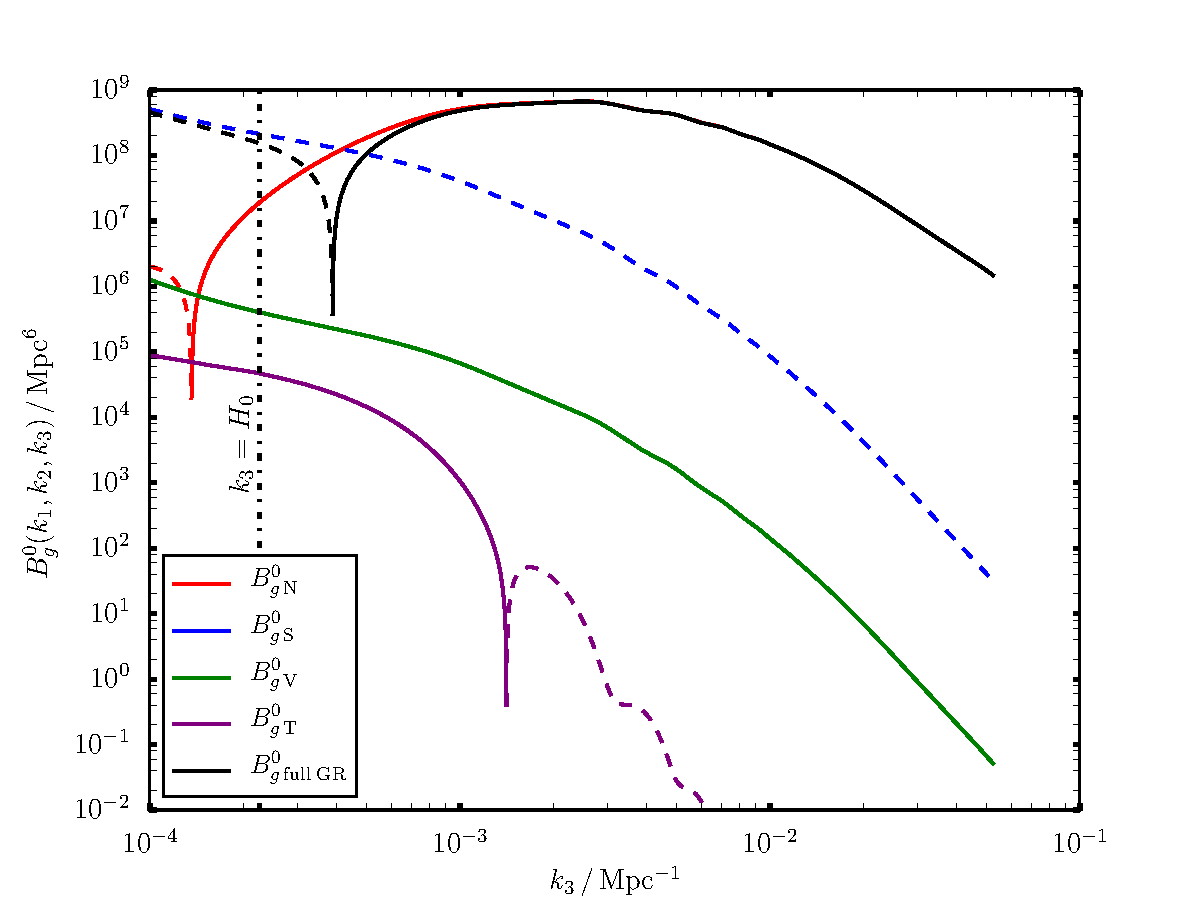
\includegraphics[width=0.9\textwidth]{fig/vectortensor_monopole.pdf}
	\caption{The separated vector, tensor, and scalar contributions to the monopole of the galaxy bispectrum, with the full GR bispectrum in black for reference. The vector and tensor modes are subdominant at a factor of about 3 smaller than the scalar contributions, except outside the Hubble radius (and where unobservable) where they grow due to their $k$-dependence and where the Newtonian contribution becomes negative as a result of the tidal bias. The tensor contributions (purple) oscillate at small scales as they pick up the BAO.}
	\label{fig:monopolevectortensor}
\end{figure}

Figure~\ref{fig:monopolevectortensor} shows that the contributions due to vector and tensor modes are small on all scales, as expected. They grow only towards the Hubble radius (indicated on the figure with a dash-dotted vertical line) due to their $k$-dependence, with the leading behaviour scaling as $(\cH/k)^2$. While the vector contribution is larger than the contribution due to the second-order tensor modes, it is still about three orders of magnitude below the scalar contribution. When the long mode $k_3$ is outside the Hubble radius (and hence unobservable) it does grow larger than the Newtonian contribution-- this is due to the tidal bias causing a sign change in the Newtonian contribution at these scales. A final thing to note is that the tensor contribution oscillates on small scales, picking up the BAO. 

As the vector and tensor modes are subdominant compared to the scalar contributions to the bispectrum, they may safely be ignored. Integrated contributions from these sources may alter this conclusion, however due to computational complexity any integrated contributions are left for future work. 



